
\documentclass[]{beamer}

\usepackage{beamerthemesplit} 
\usepackage[utf8]{inputenc}
\usepackage{algpseudocode}
\usepackage{algorithm}

\title{Sokoban Project Presentation}
\author{Andreas Sjöberg \and Andreas Gabrielsson \and Marcus Larsson}
\institute{The Predicates \\ KTH}
\date{\today}

\begin{document}

\begin{frame}
  \titlepage
\end{frame}

\section[Outline]{}

\begin{frame}
  \tableofcontents
\end{frame}

\section{Prerequisites}

\subsection{State definition}
\begin{frame}
	\frametitle{What are equivalent states?}
	\begin{itemize}
		\item{Move the boxes, not the player}
		\item{What can change?
			\pause
			\begin{itemize}
				\item{The player's position}
				\item{The boxes' positions}
			\end{itemize}
		}
	\end{itemize}
	\pause
	$$State = (Box, ReachableLocations) $$ 
\end{frame}

\subsection{Bidirectional search}
\begin{frame}
	\frametitle{Bidirectional search}
	\begin{itemize}
		\item{Forward vs. Backward solver}
		\pause
		\item{Why not use both?
			\begin{itemize}
				\item{Some map are easier to solve using either option}
				\item{Also, $2 \cdot 2^\frac{n}{2} \ll 2^n$}
			\end{itemize}
		}
	\end{itemize}
\end{frame}


\section{Algorithm description}

\begin{frame}
	\frametitle{Rough algorithm description}
	\begin{itemize}
		\item{Alternate backwards and forwards search, avoiding dead states}
		\item{When a common state is found, a solution has been found}
		\item{After a certain time, start over with new heuristics}
	\end{itemize}
\end{frame}

\subsection{Static dead lock detection}
\begin{frame}
	\frametitle{Static dead lock detection}
	\begin{itemize}
		\item{Deadlock detection is hard}
		\item{Best $\frac{Bang}{Buck}$ is to avoid trivial dead states}
	\end{itemize}
\end{frame}

\begin{frame}
	\frametitle{Algorithm for trivial deadlock detection}
	\begin{algorithmic}
		\Function{DeadPositions}{$board$}
			\For {$position \in board$}
				\State $position \gets dead$
			\EndFor
			\For {$goal \in board.goals$}
				\For {$position \in board$}
					\If {\Call{CanPullFromTo}{$goal$, $position$}}
						\State $position \gets alive$
					\EndIf
				\EndFor
			\EndFor
		\EndFunction
	\end{algorithmic}

\end{frame}
\subsection{Best-first-search}
\begin{frame}
	\frametitle{Best-first-search}
	\begin{itemize}
		\item{The state space is (almost) infinite}
		\item{We need to prioritize the order to expand nodes}
		\item{Search depth is not so important}
	\end{itemize}
\end{frame}


\subsection{Heuristics}
\begin{frame}
	\frametitle{Heuristic functions}
	\begin{itemize}
		\item{Boxes on goals}
		\item{Mobility}
		\item{Continuity}
	\end{itemize}
\end{frame}

\begin{frame}
	\frametitle{Weighing heuristics}
	\begin{columns}
	\column{0.5\textwidth}
	\begin{enumerate}
		\item{Use a reasonable start value}
		\item{Try another reasonable value}
		\item{Randomize!}
	\end{enumerate}
	\column{0.5\textwidth}
	\framebox{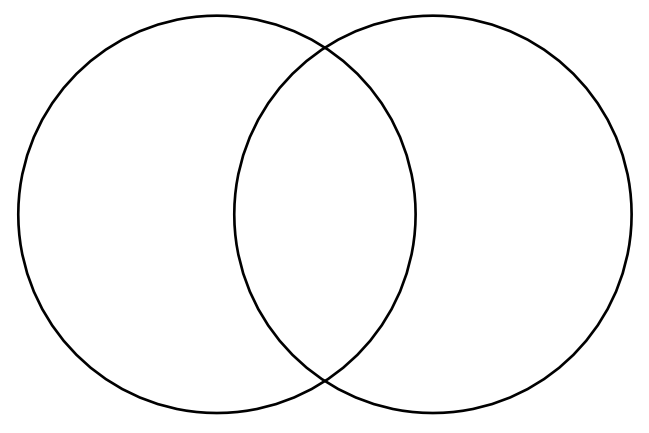
\includegraphics[width=\textwidth]{2venn}}
	\end{columns}
\end{frame}

\subsection{Building the solution}
\begin{frame}
	\frametitle{Building the solution}
	\begin{itemize}
		\item{Once solved, we have two state sequences which together form a solution}
		\item{Generate the player movements for each of these sequences}
		\item{Concatenate these for the complete solution}
	\end{itemize}
\end{frame}

\section{Improvements}
\subsection{CPU Optimizations}

\begin{frame}
	\frametitle{CPU Optimizations}
	\begin{itemize}
		\item{Wasting precious CPU cycles}
		\item{Precomputation is key!}
		\item{Precompute things that are constant throughout execution
			\begin{itemize}
				\item{Hashcode for immutables}
				\item{Neighbours to coordinates}
			\end{itemize}
		}
	\end{itemize}
\end{frame}

\subsection{Memory Optimizations}

\begin{frame}
	\frametitle{Saving Memory}
	\begin{itemize}
		\item{Avoid multiple instances of the same logical objects}
		\item{Do not store every reachable position in the state}
		\item{Remember only the positions that are relevant}
	\end{itemize}
\end{frame}

\section{Results and Conclusions}


\subsection{Performance}
\begin{frame}
	\frametitle{Performance}
	\begin{columns}
		\column{0.3\textwidth}
		\begin{itemize}
			\item{Note: This is from our final evaluation.}
			\item{Solved: 87\\ Failed: 13}
		\end{itemize}
	\column{0.7\textwidth}
		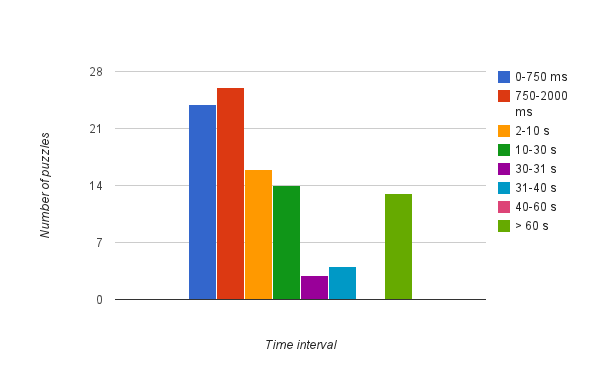
\includegraphics[width=\textwidth]{time_graph}
	\end{columns}
\end{frame}

\subsection{Conclusions}
\begin{frame}
	\frametitle{Conclusions}
	\begin{itemize}
		\item{Key features
			\begin{itemize}
				\item{Bidirectional search}
				\item{Simple deadlock detection}
			\end{itemize}
		}
		\item{Suggested improvements

			\begin{itemize}
				\item{More advanced deadlock detection}
				\item{Tunnel macros}
				\item{A systematic approach to the heuristics weights}
				\item{Pattern recognition (rooms, doors, goal zones etc.)}
			\end{itemize}
		}
	\end{itemize}
\end{frame}

\begin{frame}
	\begin{center}
		EOF
	\end{center}
\end{frame}
\end{document}
